%%%%%%%%%%%%%%%%%%%%%%%%%%%%%%%%%%%%%%%%%%%%%%%%%%%%%%%%%%%%%%%%
%%                                                            %%
%%   essentialsOfLatin, Italian translation 2017              %%
%%                                                            %%
%% From:  Henry C. Pearson, Essentials Of Latin For Beginners %%
%%        (1915, New York, American Book Company)             %%
%%                                                            %%
%%    https://archive.org/details/essentialslatin04peargoog   %%
%%                                                            %%
%% Translated by g.p.ciceri <gp.ciceri@gmail.com>             %%
%% ---------------------------------------------------------- %%
%% This translation is Licensed under                         %%
%% Creative Commons Attribution-ShareAlike 4.0 International  %%
%% https://creativecommons.org/licenses/by-sa/4.0/            %%
%%                                                            %%
%%%%%%%%%%%%%%%%%%%%%%%%%%%%%%%%%%%%%%%%%%%%%%%%%%%%%%%%%%%%%%%%

% āēīōū
% ăĕĭŏŭ




\documentclass[nols]{tufte-handout}

%\geometry{showframe} % display margins for debugging page layout

\usepackage{fontspec}
\usepackage{ifxetex}
\setmainfont[Path=./fonts/palatino-linotype/, ItalicFont=palai.ttf, BoldFont=palab.ttf]{pala.ttf}


% \defaultfontfeatures{Mapping=tex-text}
% \setromanfont[Path=./fonts/TeX-Gyre-Schola/,Mapping=tex-text]{TeX Gyre Schola}
% \setsansfont[Path=./fonts/TeX-Gyre-Heros/,Scale=MatchLowercase,Mapping=tex-text]{TeX Gyre Heros}
% \setmonofont[Path=./fonts/TeX-Gyre-Cursor/,Scale=MatchLowercase]{TeX Gyre Cursor}

\usepackage{lipsum}
\usepackage{url}
\usepackage{longtable}
\usepackage{stackengine}

\usepackage{graphicx} % allow embedded images
  \setkeys{Gin}{width=\linewidth,totalheight=\textheight,keepaspectratio}
  \graphicspath{{graphics/}} % set of paths to search for images
\usepackage{amsmath}  % extended mathematics
\usepackage{booktabs} % book-quality tables
\usepackage{units}    % non-stacked fractions and better unit spacing
\usepackage{multicol} % multiple column layout facilities
\usepackage{lipsum}   % filler text
\usepackage{fancyvrb} % extended verbatim environments
  \fvset{fontsize=\normalsize}% default font size for fancy-verbatim environments

% Standardize command font styles and environments
\newcommand{\doccmd}[1]{\texttt{\textbackslash#1}}% command name -- adds backslash automatically
\newcommand{\docopt}[1]{\ensuremath{\langle}\textrm{\textit{#1}}\ensuremath{\rangle}}% optional command argument
\newcommand{\docarg}[1]{\textrm{\textit{#1}}}% (required) command argument
\newcommand{\docenv}[1]{\textsf{#1}}% environment name
\newcommand{\docpkg}[1]{\texttt{#1}}% package name
\newcommand{\doccls}[1]{\texttt{#1}}% document class name
\newcommand{\docclsopt}[1]{\texttt{#1}}% document class option name
\newenvironment{docspec}{\begin{quote}\noindent}{\end{quote}}% command specification environment

% concetti morfosintattici
\usepackage{xspace} 
\newcommand{\noun}{\textsc{sostantivo}\xspace}
\newcommand{\nouns}{\textsc{sostantivi}\xspace}
\newcommand{\adject}{\textsc{aggettivo}\xspace}
\newcommand{\adjects}{\textsc{aggettivi}\xspace}
\newcommand{\gnumber}{\textsc{numero}\xspace}
\newcommand{\gnumbers}{\textsc{numeri}\xspace}
\newcommand{\gender}{\textsc{genere}\xspace}
\newcommand{\genders}{\textsc{generi}\xspace}
\newcommand{\gcase}{\textsc{caso}\xspace}
\newcommand{\gcases}{\textsc{casi}\xspace}
\newcommand{\tense}{\textsc{tempo}\xspace}
\newcommand{\mood}{\textsc{modo}\xspace}
\newcommand{\gverb}{\textsc{verbo}\xspace}
\newcommand{\gverbs}{\textsc{verbi}\xspace}
\newcommand{\adjective}{\textsc{aggettivo}\xspace}
\newcommand{\nom}{\textsc{nom}\xspace}
\newcommand{\gen}{\textsc{gen}\xspace}
\newcommand{\dat}{\textsc{dat}\xspace}
\newcommand{\acc}{\textsc{acc}\xspace}
\newcommand{\voc}{\textsc{voc}\xspace}
\newcommand{\abl}{\textsc{abl}\xspace}
\newcommand{\gexit}{\textsc{uscita}\xspace}
\newcommand{\gexits}{\textsc{uscite}\xspace}
\newcommand{\declinazione}{\textsc{declinazione}\xspace}
\newcommand{\masc}{\textsc{maschile}\xspace}
\newcommand{\femm}{\textsc{femminile}\xspace}
\newcommand{\neut}{\textsc{neutro}\xspace}

\newcommand{\indic}{\textsc{indicativo}\xspace}
\newcommand{\imper}{\textsc{imperativo}\xspace}
\newcommand{\gcong}{\textsc{congiuntivo}\xspace}
\newcommand{\ott}{\textsc{ottativo}\xspace}
\newcommand{\partic}{\textsc{participio}\xspace}
\newcommand{\infin}{\textsc{infinito}\xspace}

\newcommand{\pres}{\textsc{presente}\xspace}
\newcommand{\imperf}{\textsc{imperfetto}\xspace}
\newcommand{\aor}{\textsc{aoristo}\xspace}
\newcommand{\fut}{\textsc{futuro}\xspace}
\newcommand{\perf}{\textsc{perfetto}\xspace}
\newcommand{\pperf}{\textsc{piuccheperfetto}\xspace}

\newcommand{\sing}{\textsc{singolare}\xspace}
\newcommand{\plur}{\textsc{plurale}\xspace}
\newcommand{\dual}{\textsc{duale}\xspace}

\newcommand{\si}{\textsc{sing}\xspace}
\newcommand{\pl}{\textsc{plur}\xspace}
\newcommand{\du}{\textsc{dual}\xspace}

\newcommand{\att}{\textsc{attivo}\xspace}
\newcommand{\med}{\textsc{medio}\xspace}
\newcommand{\pass}{\textsc{passivo}\xspace}
\newcommand{\medpass}{\textsc{medio-passivo}\xspace}


% italianitudini
\renewcommand{\figurename}{Figura}
\renewcommand{\tablename}{Tabella}
\renewcommand{\contentsname}{Indice}

% fix per un qualche problema
\ifxetex
  \newcommand{\textls}[2][5]{%
    \begingroup\addfontfeatures{LetterSpace=#1}#2\endgroup
  }
  \renewcommand{\allcapsspacing}[1]{\textls[15]{#1}}
  \renewcommand{\smallcapsspacing}[1]{\textls[10]{#1}}
  \renewcommand{\allcaps}[1]{\textls[15]{\MakeTextUppercase{#1}}}
  \renewcommand{\smallcaps}[1]{\smallcapsspacing{\scshape\MakeTextLowercase{#1}}}
  \renewcommand{\textsc}[1]{\smallcapsspacing{\textsmallcaps{#1}}}
\fi

% too many float...
\extrafloats{100}
% āēīōū
% ăĕĭŏŭ

\title{Essentials Of Latin. Elementi di Latino. \newline Introduzione, prime nozioni.}

\author[gpciceri]{a cura di Milagathòs: Milo's help to enjoy humanities.}

\date{20 Gennajo 2017} % without \date command, current date is supplied


\begin{document}

\hyphenation{co-niu-ga-zio-ne}

\maketitle% this prints the handout title, author, and date

\begin{marginfigure}[-2.0cm]
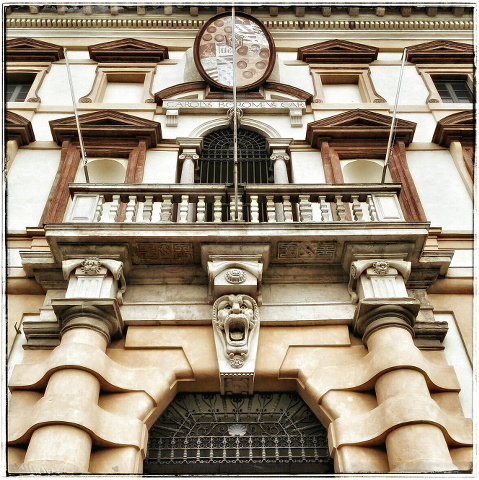
\includegraphics{smallthumb-lesson_I.jpeg}
\setfloatalignment{b}
\end{marginfigure}


\begin{abstract}
\noindent
Queste lezioni riprendono il testo introduttivo al Latino di Pearson\cite{pearson1915}, del quale seguono la numerazione; la struttura di ogni lezione è piuttosto regolare: inizia con \textsc{cenni di morfologia e di sintassi latina}, seguita da un \textsc{piccolo vocabolario} per il lessico; ci sono infine vari \textsc{esercizi} di traduzione e di composizione latina.

\bigskip
\noindent
Introduzione. Alfabeto, dittonghi, sillabazione, quantità, vocali aperte e chiuse, flessioni nominali e verbali, radice e tema del nome.
\end{abstract}

%\printclassoptions

\newthought{1.} Queste prime nozioni vanno lette ed utilizzate poi come riferimento per quanto verrà spiegato in seguito. I vocabili alle sezioni 9. e 21. vanno letti e ripetuti ad alta voce.  

\newthought{2. Alfabeto.} L'alfabeto latino è come quello Italiano, senza \textit{j, w}. La lettera \textit{i} è usata sia come vocale che come insonante: è una consonante quando, nella stessa sillaba, viene prima di una vocale, come in \textbf{iunior}.

\newthought{3. Vocali e Consonanti.} Le vocali sono \textbf{a, e, i, o, u} (lunghe o brevi). Le altre lettere sono consonanti.

\newthought{4. Dittonghi.} I dittonghi sono combinazioni di due vocali che sono pronunciate come un'unica sillaba. In Latino i dittonghi sono \textbf{ae, oe, au, eu, ui}.

\newthought{5. Pronuncia delle vocali lunghe.} Una vocale lunga viene pronunciata per un tempo all'incirca doppio della corrispondente vocale breve:
\begin{itemize}
\item[\textsc{ā}] come la \textit{a} dell'inglese \textit{father}.  
\item[\textsc{ē}] come la \textit{e} dell'inglese \textit{prey}. 
\item[\textsc{ī}] come la \textit{i} dell'inglese \textit{machine}.  
\item[\textsc{ō}] come la \textit{o} dell'inglese \textit{note}.  
\item[\textsc{ū}] come le \textit{oo} dell'inglese \textit{root}.  
\end{itemize}

\newthought{6. Pronuncia delle vocali brevi.} Come segue:
\begin{itemize}
\item[\textsc{ă}] come la prima \textit{a} dell'inglese \textit{ahà}.  
\item[\textsc{ĕ}] come la \textit{e} dell'inglese \textit{step}. 
\item[\textsc{ĭ}] come la \textit{i} dell'inglese \textit{pit}.  
\item[\textsc{ŏ}] come la \textit{o} dell'inglese \textit{or}.  
\item[\textsc{ŭ}] come la \textit{u} dell'inglese \textit{pull}.  
\end{itemize} 

\newthought{7. Pronuncia (classica, o restituta) delle consonanti.} La maggior parte delle consonanti si pronunciano come in italiano, ma vale la pena di tenere presente (gli esempi sono quelli del testo originale, che spiega la pronuncia (classica) a studenti di lingua inglese): 
\begin{itemize}
\item[\textsc{c} e \textsc{g}] sono sempre dure, come nell'inglese \textit{come} e \textit{go}.  
\item[\textsc{s}] sibilante come nell'inglese \textit{sin}, mai come una \textit{z} (nell'inglese \textit{ease}). 
\item[\textsc{i}] se consonante, come la \textit{y} dell'inglese \textit{yes}.  
\item[\textsc{t}] sempre dura, come nell'inglese \textit{tin}.  
\item[\textsc{v}] come la \textit{w} dell'inglese \textit{wine}.  
\item[\textsc{ch}] come la \textit{ch} dell'inglese \textit{chorus}.  
\item[\textsc{ph}] come la \textit{ph} dell'inglese \textit{alphabet}.  
\item[\textsc{qu}] come nell'inglese \textit{kw}. 
\item[\textsc{ti}] come è scritto (nella pronuncia scolastica, invece, il gruppo \textbf{ti} non accentato di solito si pronuncia \textit{zi}).  
\end{itemize} 

\newthought{8. Pronuncia (classica) dei dittonghi.} Come segue: 
\begin{itemize}
\item[\textsc{ae}] come la \textit{ai} dell'inglese \textit{aisle}. 
\item[\textsc{oe}] come la \textit{oi} dell'inglese \textit{toil}. 
\item[\textsc{ui}] come nell'inglese \textit{we}.  
\item[\textsc{au}] come la \textit{ou} dell'inglese \textit{house}. 
\item[\textsc{eu}] come nell'inglese \textit{éh-oo}.  
\item[\textsc{ei}] come la \textit{ei} dell'inglese \textit{eight}.  
\end{itemize} 



\newthought{9.} Pronuncia con cura le seguenti parole:
\begin{fullwidth}
\begin{table}[!htbp]
  \centering
  \begin{tabular}{l l l l l l l}
    %\toprule
	hi & iam & tot & me & genus & -que & cui \\
	ad & vis & sic & quia & coepit & vir & aeger \\
	ita & quis & haec & causa & regno & mensae & \\
    %\bottomrule
  \end{tabular}
  %\caption[bottom]{}
  \label{tab:normaltab}
  %\zsavepos{pos:normaltab}
\end{table}
\end{fullwidth}

\newthought{10. Sillabe.} Una sillaba è composta da una sola vocale (o da un dittongo) assieme a una o più consonanti, che la precedono o seguono. Da questo si deduce che una parola ha tante sillabe quante sono le sue vocali isolate (o i suoi dittonghi): come in \textbf{ae-dì-fi-co}, \textit{io costruisco}.

\newthought{11.} Tranne che nelle parole composte (vedi poi 13.), una singola consonante tra due vocali (o dittonghi) va considerata assieme alla seconda vocale per formare una sillaba, come in \textbf{a-mì-cus}, \textit{amico} e in \textbf{di-xit}, \textit{egli disse}.

\newthought{11.} Se ci sono due o più consonanti tra due vocali (o dittonghi), la divisione in sillabe viene fatta prima dell'ultima consonante: come in \textbf{hòs-pes}, \textit{ospite}, \textbf{dic-tus}, \textit{detto}, \textbf{sanc-tus}, \textit{santo}, \textbf{cog-nos-co}, \textit{riconosco}. Fanno eccezione la \textbf{l} e la \textbf{r} che \textit{attraggono} la consonante che le precede a costituire sillaba con la seconda vocale: come in \textbf{de-mons-tro}, \textit{dimostro},  \textbf{pu-bli-cus}, \textit{pubblico}.

\newthought{13.} Le parole composte sono divise in sillabe secondo quelle delle loro parole componenti: come in \textbf{ad-est} (\textbf{ad}, \textit{vicino}; \textbf{est}, \textit{è}), \textit{è presente}.

\newthought{14.} Le consonanti doppie sono separate, come in \textbf{pu-el-la}, \textit{ragazza}.

\newthought{15. Ultima, Penultima, Terzultima} L'ultima sillaba di una parola viene detta \textit{l'ultima}; quella prima dell'ultima viene detta \textit{la penultima}; quella prima della penultima viene detta \textit{la terzultima}.

\newthought{16. Quantità.} Le vocali possono essere lunghe \textbf{(āēīōū)} o brevi \textbf{(ăĕĭŏŭ)}. Di solito si segnano solo le vocali lunghe, nel senso che se una vocale non è segnata si intende sia breve: in letteratura non sempre però si segue questa convenzione. 

\newthought{17. Regole generali sulle quantità delle vocali}
\begin{itemize}
\item[\textsc{1.}] Una vocale prima di un'altra vocale o di \textbf{h} è corta, come in \textbf{cō-pĭa}, \textit{abbondanza}. 
\item[\textsc{2.}] Le vocali che risultano da una contrazione sono lunghe, come in \textbf{cō-gō (cŏăgō)}, \textit{raccolgo}. 
\item[\textsc{3.}] Le vocali prima di \textbf{nf, ns, nct, ncs} sono lunghe, come in \textbf{īnferō}, \textit{porto dentro}, \textbf{īnsanūs}, \textit{pazzo}.  
\item[\textsc{4.}] I dittonghi sono lunghi: \textbf{cāūsa}, \textit{la causa}. 
\end{itemize} 

\newthought{18. Sillaba lunga per natura.} Una sillaba che contiene una vocale lunga o un dittongo viene detta \textit{lunga per natura}, come in \textbf{lē-gēs}, \textit{le leggi}; \textbf{aē-dēs}, \textit{il tempio}. 

\newthought{18. Sillaba lunga per posizione.} Una sillaba che contiene una vocale corta seguita da due o più consonanti, o da una tra \textbf{x} o \textbf{z}, viene detta \textit{lunga per posizione}. Tuttavia la vocale corta viene pronunciata corta, come in  \textbf{vocant}, \textit{chiamano}; \textbf{dux}, \textit{condottiero};. 

\newthought{20. L'Accento.} I seguenti principi determinano su quale sillaba della parola vada a cadere l'accento:
\begin{itemize}
\item[\textsc{1.}] \textit{L'ultima} non è mai accentata. 
\item[\textsc{2.}] Nelle parole di due sillabe, l'accento cade sulla \textit{penultima}, come in \textbf{témplum}, \textit{tempio}. 
\item[\textsc{3.}] Nelle parole di più di due sillabe, l'accento cade sulla \textit{penultima} quando questa è \textit{lunga per natura o per posizione}, come in \textbf{amàre}, \textit{amare}; altrimenti sulla \textit{terzultima}, come in \textbf{mìttere}, \textit{mandare}.  
\item[\textsc{4.}] Le enclitiche: alcune parole monosillabiche, come \textbf{-ne} (particella interrogativa) e \textbf{-que} (congiunzione), sono talmente collegate alla parola che le precede che sono pronunciate assieme a quest'ultima: in questo caso l'accento finisce sull'ultima sillaba della parola cui sono collegate, come in \textbf{amàtne}, \textit{ama egli?}; \textbf{hominésque}, \textit{e gli uomini} . 
\end{itemize} 

\begin{marginfigure}
\includegraphics{meme-lesson_Intro.jpeg}
\setfloatalignment{b}
\end{marginfigure}

% āēīōū
% ăĕĭŏŭ


\newthought{21.} Dividi in sillabe, segna l'accento e pronuncia con cura le seguenti parole:
\begin{fullwidth}
\begin{table}[!htbp]
  \centering
  \begin{tabular}{l l l l}
    %\toprule
	inīquus & vincam & aedificium & gladiō \\
	grātiae & fīlius & coepērunt & cuius \\
	huic & īdem & fīliusque & quae \\
	monēre & vērō & mēnsārum & faciēbam \\
	facere & aegritūdō & pugnābō & laudābimus \\
    %\bottomrule
  \end{tabular}
  %\caption[bottom]{}
  \label{tab:normaltab}
  %\zsavepos{pos:normaltab}
\end{table}
\end{fullwidth}

\newthought{22. Parti del discorso.} Sono le stesse dell'italiano, tranne per l'articolo, che in latino manca: sono quindi nome, aggettivo, pronome, verbo, avverbio, preposizione, congiunzione, interiezione.

\newthought{23. Flessioni.} Sono le modifiche che avvengono alle parole per indicare le loro relazioni grammaticali con il resto della frase. Le flessioni di nomi, aggetti e pronomi sono dette \textit{declinazioni}; quelle dei verbi sono dette \textit{coniugazioni}.

\newthought{24. Declinazioni.} Nomi, aggettivi e pronomi si declinano secondo sei casi, diversi per la \textit{terminazione del caso}, o \textit{uscita}:

\begin{itemize}
\item[\textsc{1.}] \textit{Nominativo}, il caso del soggetto.  
\item[\textsc{2.}] \textit{Genitivo}, il caso del complemento di specificazione.  
\item[\textsc{3.}] \textit{Dativo}, il caso del complemento di termine (oggetto \textit{indiretto} dell'azione espressa dal verbo).  
\item[\textsc{4.}] \textit{Accusativo}, il caso del complemento oggetto \textit{diretto} dell'azione espressa dal verbo.
\item[\textsc{5.}] \textit{Vocativo}, il caso del discorso diretto.  
\item[\textsc{6.}] \textit{Ablativo}, questo caso esprime diverse relazioni avverbiali, sia senza che con alcune preposizioni. Il Complemento di Mezzo, ad esempio, si esprime di norma con l'ablativo semplice. 
\end{itemize}
I nomi in latino sono divisi in cinque declinazioni, distinte l'una dall'altra per la differente uscita del genitivo singolare.

\newthought{25. Radice e Tema.} La \textbf{radice} è quella forma che stabilisce in generale il significato della parola. La lettera finale della radice, detta \textit{caratteristica della radice}, spesso scompare o viene cambiata prima della terminazione del caso. Si trova sempre nel genitivo plurale della parola tranne che nelle radici in \textbf{-o-}, dove questa \textbf{o} è allungata. Il \textbf{tema} (quella parte del nome che rimane invariata nella declinazione, e alla quale si aggiungono direttamente le uscite dei casi) si forma a partire dalla radice senza la caratteristica, oppure togliendo l'uscita dal genitivo singolare. 

\newthought{26. Coniugazione.} I verbi in latino hanno:
\begin{itemize}
\item[\textsc{1.}] Tre modi finiti: Indicativo, Congiuntivo, Imperativo; cinque modi indefiniti: Infinito, Participio, Supino, Gerundio e Gerundivo.  
\item[\textsc{2.}] Sei tempi: Presente, Imperfetto, Futuro, Perfetto, Piuccheperfetto, Futuro Anteriore (o Futuro Perfetto).  
\item[\textsc{3.}] Due diatesi: Attiva e Passiva.  
\item[\textsc{4.}] Tre persone: Prima, Seconda e Terza.
\item[\textsc{5.}] Due numeri: Singolare e Plurale.  
\end{itemize}

\newthought{27. Genere.} In latino ci sono tre generi: Maschile, Femminile e Neutro. Nei soli nomi di persona il genere è determinato dal sesso. In tutti gli altri casi il genere è determinato dal significato del nome o dalla terminazione del nominativo (in questo caso si dice \textit{Genere Grammaticale}. 

\newthought{28. Regole generali sul riconoscimento del genere.}
\begin{itemize}
\item[\textsc{1.}] I nomi che denotano maschi e i nomi di \textit{fiumi, venti e mesi} sono maschili:  
\textbf{nauta}, \textit{marinaio}; 
\textbf{Tiberis}, \textit{il (fiume) Tevere}; 
\textbf{Caesar}, \textit{Cesare}; 
\textbf{aquilo}, \textit{vento del nord}; 
\textbf{Ianuarius}, \textit{Gennaio}.  
\item[\textsc{2.}] I nomi che denotano femmine e i nomi di \textit{paesi, città e alberi} sono femminili: 
\textbf{filia}, \textit{figlia}; 
\textbf{Italia}, \textit{l'Italia}; 
\textbf{Athenae}, \textit{Atene}; 
\textbf{pirus}, \textit{il pero} l'albero delle pere.  
\item[\textsc{3.}] I nomi indeclinabili sono neutri: \textbf{nihil}, \textit{nulla};.  
\end{itemize}

\begin{figure*}[!b]
  %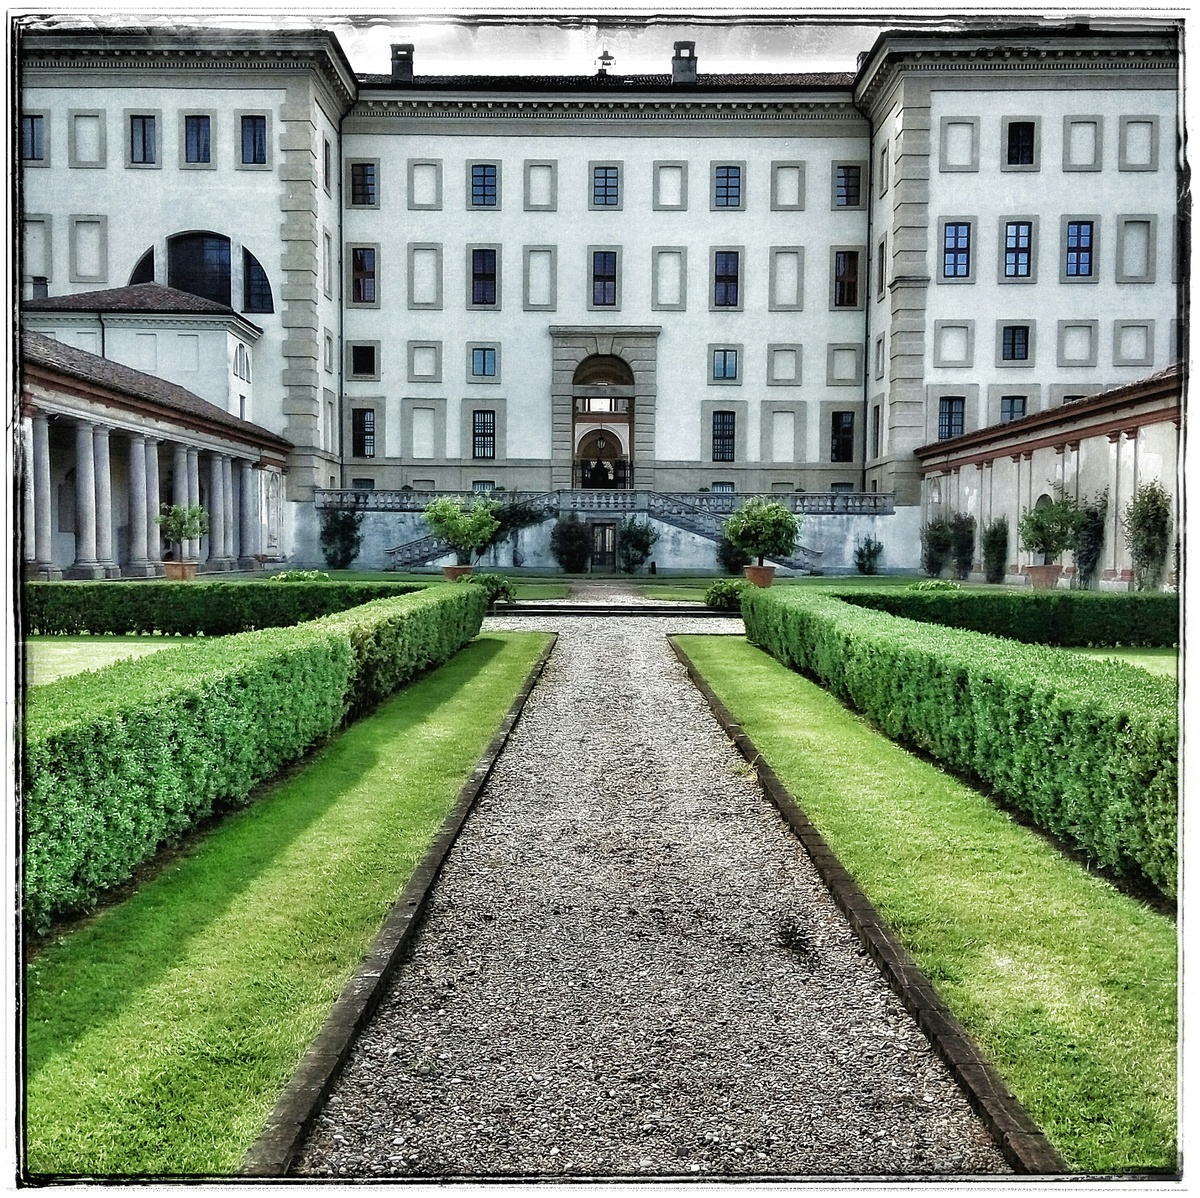
\includegraphics{thumb-lesson_Intro.jpeg}
  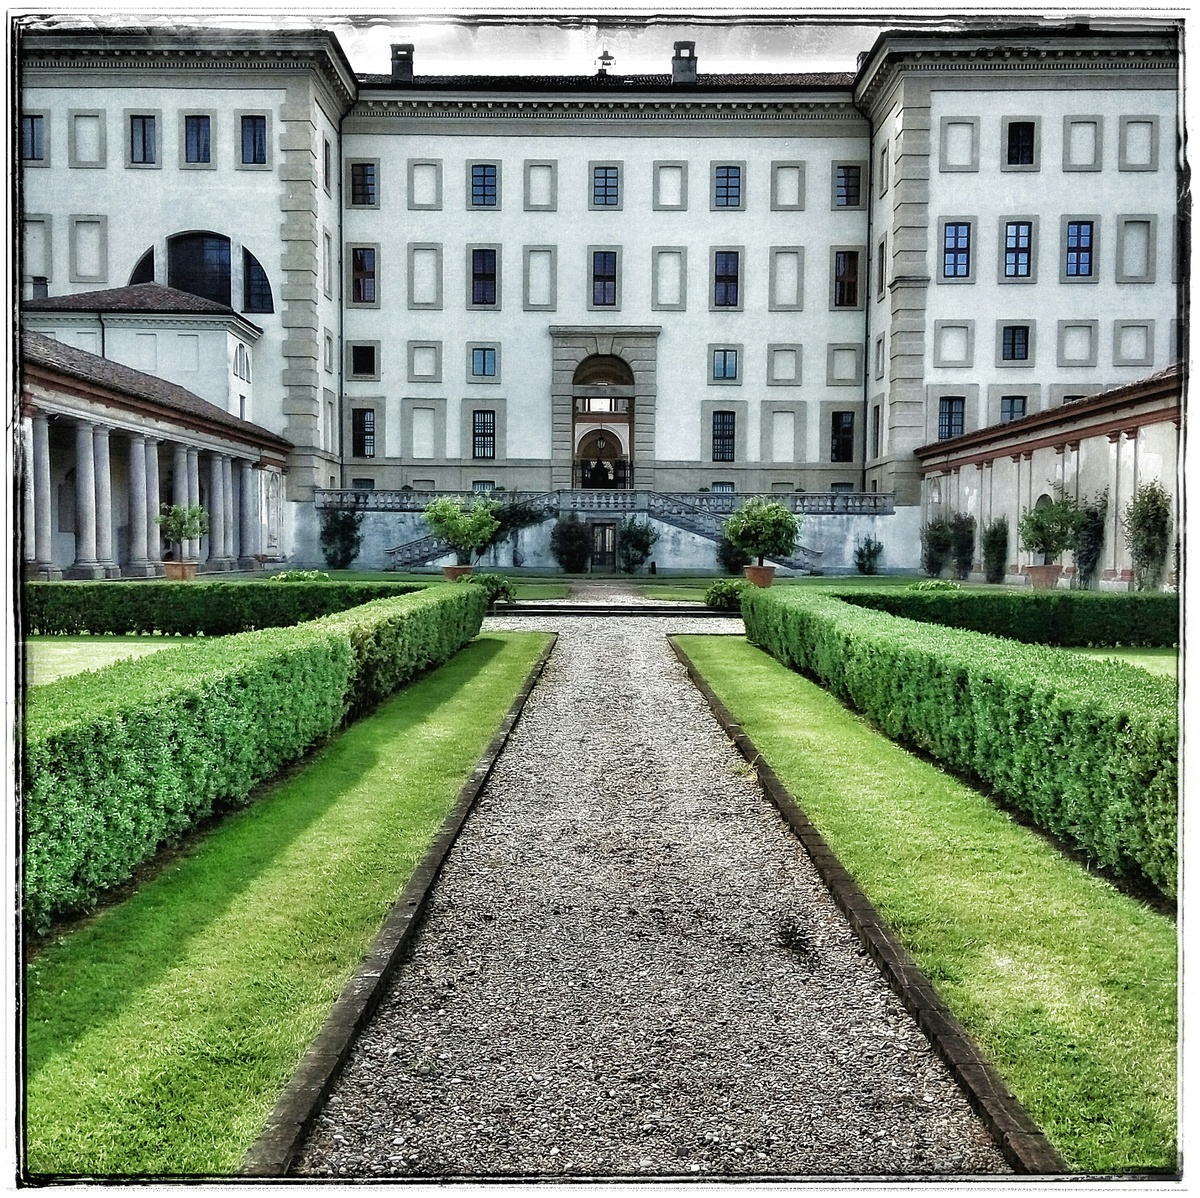
\includegraphics[width=0.8\linewidth]{thumb-lesson_Intro.jpeg}
  %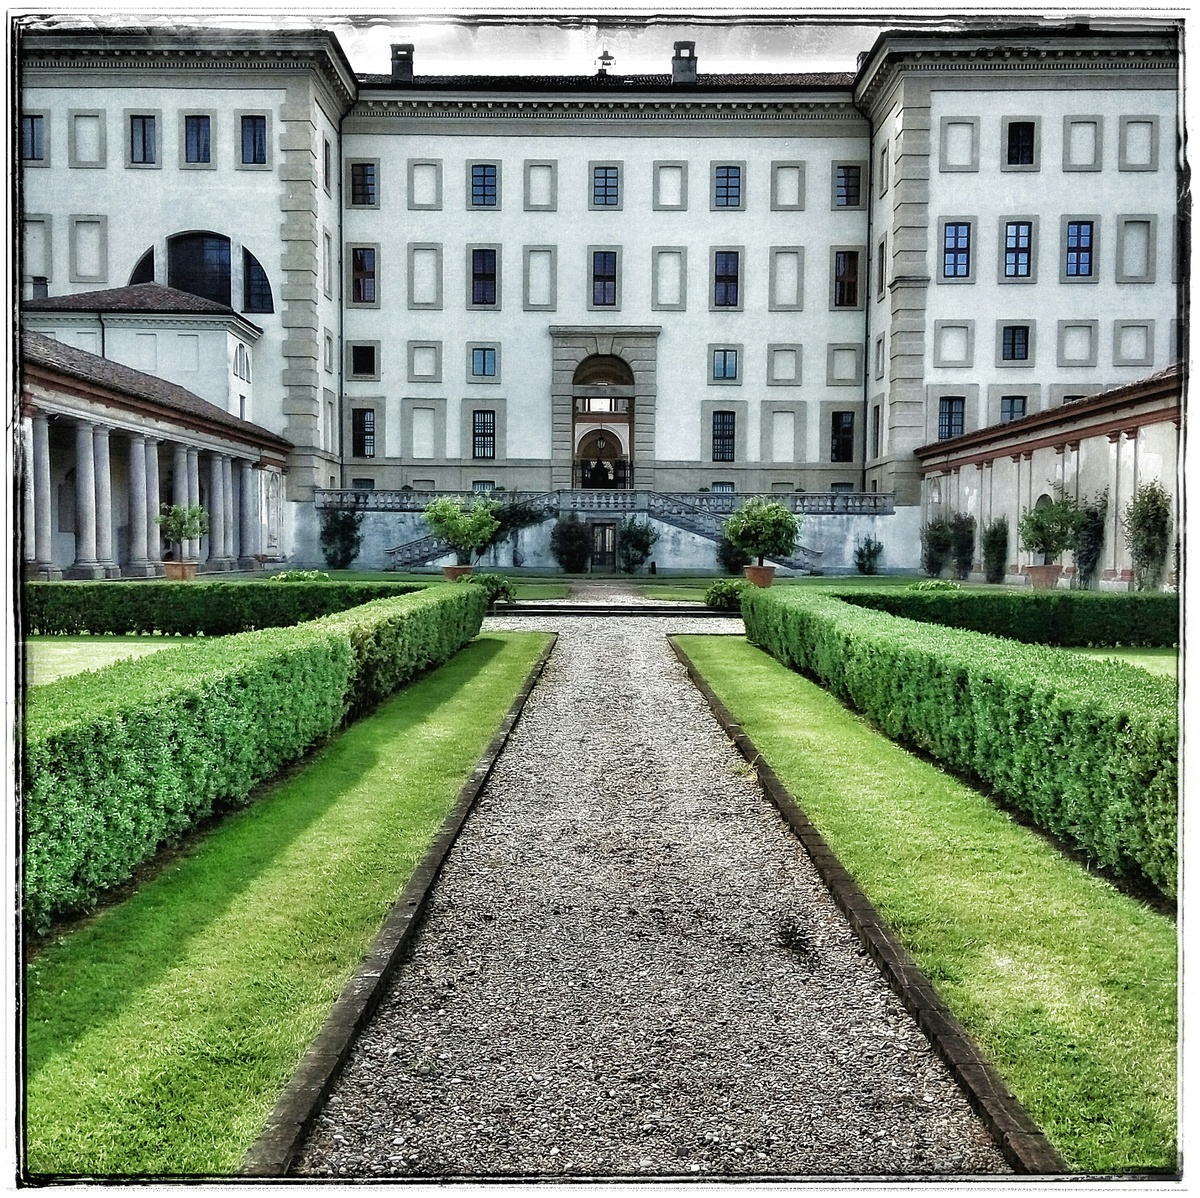
\includegraphics{thumb-lesson_Intro.jpeg}
  \caption{Pavia: Almo Collegio Borromeo, dal giardino.}
  \label{fig:textfig}
  %\zsavepos{pos:textfig}
  %\setfloatalignment{b}
\end{figure*}

 

\nobibliography{latinBiblio}
\bibliographystyle{alpha}


\end{document}
